\pagestyle{empty}
\cleardoublepage
\pagestyle{fancy}

\chapter{METODOLOGIA}\label{cap3}

\section*{WEB SCRAPING}

O surgimento da internet, em particular a Web (\emph{Web Wide Word}) trouxe um crescimento exponencial nas disposições de informações. Embora muitas dessas informações sejam úteis, elas raramente estão de uma forma que podemos utilizá-las, pois ainda é comum pessoas gastarem horas na coleta manual de dados de páginas da web.
Especificamente, apesar de disponibilidade, poucos trabalhos acadêmicos em Economia utilizam desta fonte de dados para análise econômica empírica. Tal característica pode ser dada pela dificuldade dos pesquisadores na área em lidar com linguagem de programação que demandam maior conhecimento de computação. Em recente publicação, \citet{varian2014big} salienta que as técnicas utilizadas na Ciência da Computação e outras áreas correlatas para manipular e analisar dados, têm muito a oferecer. \citet{varian2014big} defende que economistas deveriam conhecer melhor esses métodos e usá-los em seus trabalhos. Além disso, \citet{varian2014big} cita a comumente colaboração entre os departamentos de Ciência da Computação e Estatística nas universidades dos EUA. Porém, o autor espera que em um futuro próximo os estudantes de econometria tenham maior colaboração com esses perfis. 

Uma metodologia que facilita o processo de coleta de dados da web é conhecida como \emph{web scraping} que envolve escrever algoritmos que executam automaticamente o que nós fazemos manualmente quando navegamos por uma página de um site de e-commerce, por exemplo. Outro ponto favorável é a pouca necessidade de conhecimentos prévios de programação. 

Segundo \citet{manning2008introduction} \emph{web scraping} é o processo de tirar informações desestruturadas de páginas da web e transformá-las em informações estruturadas que podem ser usadas para análise.  Pelo fato do processo ser tão genérico, é difícil dizer quando o primeiro web scraper foi escrito. Assim, como \citet{cavallo2010scraped}, apresenta-se o \emph{web scraping} como uma alternativa para acessar preços de sites de supermercados, farmácias, postos de gasolina, bancos, imobiliárias, companhia de energia elétrica, lojas de e-commerce, lojas de roupas e calçados, consertos em geral, plano de saúde, escolas particulares, cursos de línguas, entre outros. 

A tecnologia para coletar os preços é simples. A maior parte das páginas são construídas usando uma linguagem de codificação estruturada chamada de \emph{HyperText Markup Language} (HTML). Este código tem “\emph{tags}”, tais como $<center>$ e $<bold>$, que determinam o estilo e localização do texto em uma página. Estas \emph{tags} tendem a permanecer constantes ao longo do tempo, uma vez que proporcionam um “\emph{look and feel}” distinto para cada página. Por contraste, a informação dentro dessas \emph{tags}, tais como preço de produtos, mudam ao longo do tempo. O software de \emph{scraping} pode ser ensinado a utilizar as \emph{tags} em HTML pata localizar informações relevantes sobre um produto e guarda-las em um banco de dados. A repetição desse processo todos os dias produz um banco de dados em formato de painel com um registro por produto por dia. Em adição, o endereço da página (URL) onde cada produto é localizado pode ser usado para classificar produtos em categorias padronizadas. 

Na figura ~\ref{fig:01}, mostramos como o processo de coletar os preços ocorrerá:

\begin{figure}[htbp]
  \centering
  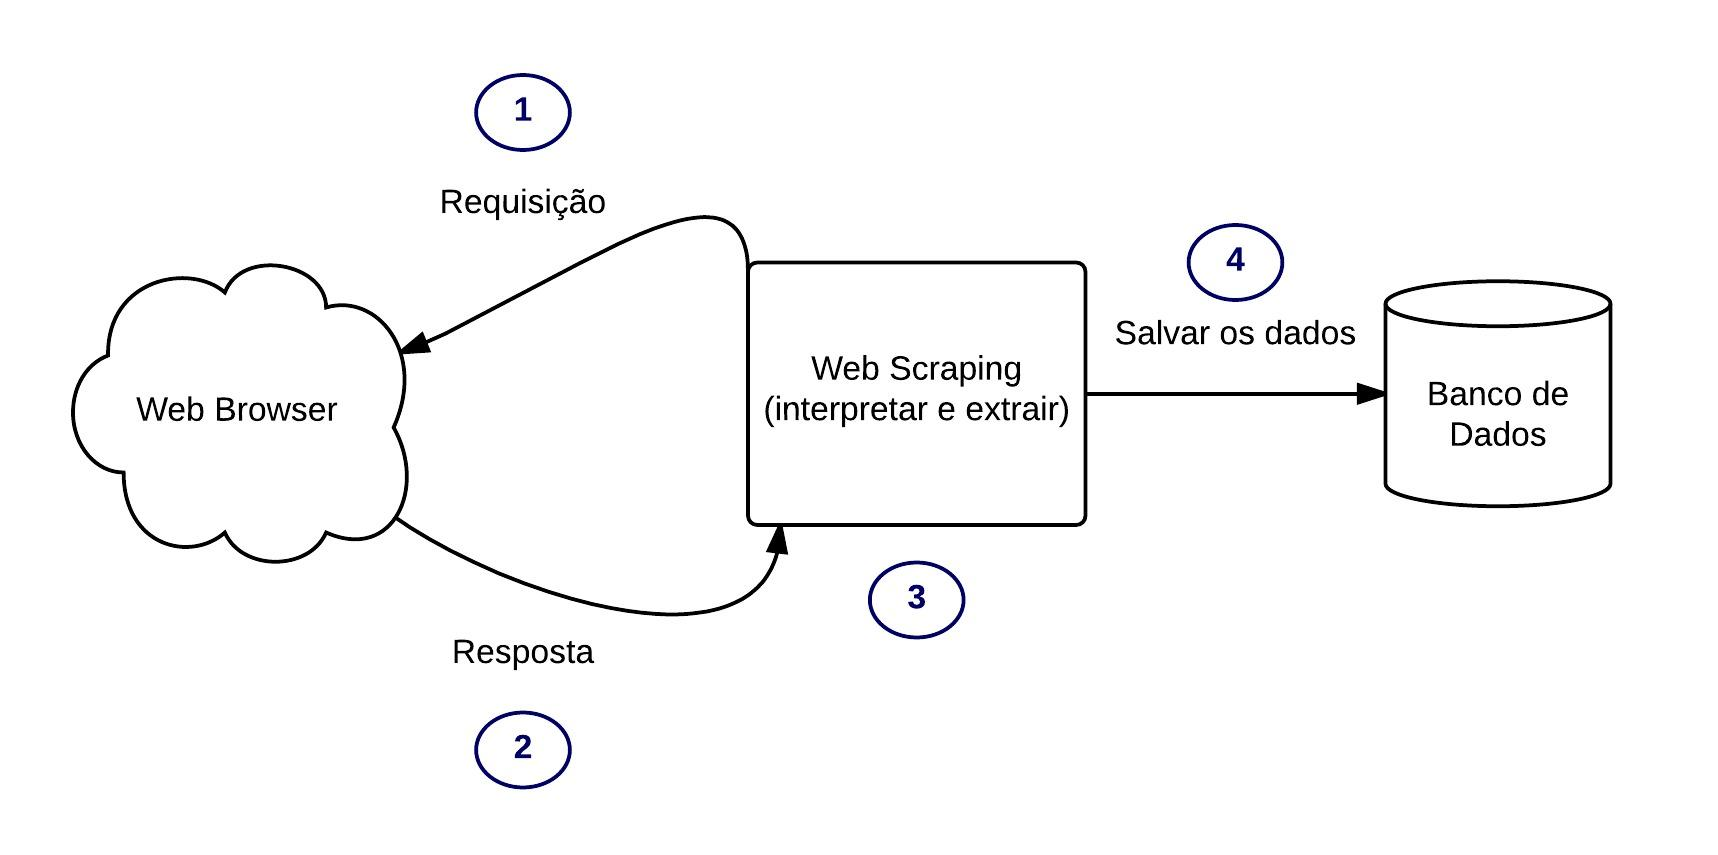
\includegraphics[width=\textwidth]{WebScraping}
  \caption[Figura Simples]{Figura abstrata simples com largura igual à do texto}
  \label{fig:01}
\end{figure}

Segundo \citet{cavallo2010scraped}, preços coletados da internet possuem duas desvantagens: Primeiro, percentual menor de empresas disponibiliza seus produtos e preços na internet em comparação com as lojas físicas. Tal limitação pode ser minimizada ao longo do tempo com uma maior oferta de produtos e serviços na internet. Segundo, os preços coletados da internet não incluem informações sobre as quantidades vendidas o que impede de obter market share e estimativas de elasticidade.

  Não obstante, \citet{cavallo2010scraped} apresenta algumas vantagens dos preços coletados da internet que os fazem uma fonte única de informação para análise de rigidez nos preços. Primeiro, pode-se obter preços diários para os produtos e serviços e por conseguinte, reduzir medidas de erro em relação à frequência de cálculo da inflação, analisar promoções de produtos, controles e sincronização nos preços. Segundo, os dados estão disponíveis para vários países, com maior facilidade de acesso e possibilidade de comparação entre países. Terceiro, existem informações detalhadas sobre cada produto e não há substituições forçada de itens como ocorre em estatísticas oficiais de inflação. Por fim, preços coletados da internet estão viáveis em tempo real, sem qualquer atraso para acessá-los. Isto pode ser usado para providenciar estimativas de rigidez nos preços em tempo real.
  
  \section*{ÍNDICE DE PREÇOS ONLINE}
  
%   Para calcular o índice de preços online que será comparado com o Índice Nacional de Preços ao Consumidor Amplo (IPCA) Índice Nacional de Preços ao Consumidor (INPC) divulgados pelo Instituto Brasileiro de Geografia e Estatística (IBGE), utilizaremos a abordagem proposta por \citet{cavallo2010scraped}.
%   
%   Assim, o índice de preços usa a combinação de dados online e as estruturas de ponderação oficiais do IBGE para as categorias da “cesta de mercadorias”\footnote[1]{Segundo o IBGE (2012) os índices constituem uma medida síntese de movimento de preços de um conjunto de bens e serviços, chamado “cesta de mercadorias”, representativo de um determinado grupo populacional, em certo período de tempo} de cada índice de inflação. Dados diários serão utilizados para construir o índice de preços online o que é útil para observar padrões de curto prazo nos dados que ajudam a validar as informações online. 
% 
%   O índice de preço online será calculado utilizando os preços de todos os produtos disponíveis para compra em cada site. Isto implica que a cesta de bens muda dinamicamente ao longo do tempo podendo um produto aparecer ou desaparecer da cesta a qualquer momento devido à disponibilidade ou indisponibilidade no site. Além disso, o número de preços por produto tende a ser muito maior o que os coletados usualmente pelos órgãos governamentais. 
% Para construir o índice, mudanças de preço são calculadas em nível de produto, então as médias dentro das categorias usando média geométrica ponderada e finalmente agregado entre categorias com uma média aritmética ponderada. Em particular, o primeiro passo é obter a média geométrica ponderada das mudanças nos preços na categoria $j$ para cada dia $t$:

\begin{equation} \label{eq:01}
R_{t,t-1}^{j}=\prod_{i}{{\left(\frac{{p}_{t}^{i}}{{p}_{t-1}^{i}}\right)}^{\sfrac{1}{{n}_{j,t}}}} 
\end{equation}





